\documentclass{article}
\usepackage[T1]{fontenc}
\usepackage{lmodern}
\usepackage{graphicx}
\usepackage{amsmath,amssymb}
\usepackage[a4paper,margin=2cm]{geometry}
\usepackage[absolute,overlay]{textpos}
\setlength{\TPHorizModule}{1mm}
\setlength{\TPVertModule}{1mm}
\usepackage[indonesian]{babel}
\usepackage{hyperref}
\setlength{\emergencystretch}{2em}
% unit: Halaman 81

\begin{document}

% === Halaman 81 (llm) ===

\textbf{Step 1:} Tentukan parameter masukan (key, nonce, counter)

\textbf{Step 2:} Inisialisasi matriks \textit{state} berukuran $4 \times 4$, setiap elemen matriks berukuran 1 word, 1 word = 32 bit. Total ukuran matriks $16 \times 32 \text{ bit} = 512 \text{ bit}$. \textit{State} berisi konstanta ('expand 32-byte k'), \textit{key}, \textit{counter}, dan \textit{nonce} dengan pengaturan letak sebagai berikut:

\vspace{10mm}

\textbf{Catatan:} Di dalam kdoe program, matriks \textit{state} dinyatakan sebagai sebuah larik $\text{in}[0..15]$

% deskripsi: Diagram matriks state Salsa20 yang menunjukkan indeks elemen (0-15) dan pemetaan tata letak konstanta, key, nonce, dan posisi (counter) dalam matriks 4x4.
% bbox normalisasi: [0.1060, 0.4250, 0.6950, 0.8550]
\begin{textblock*}{123.69mm}(22.26mm,126.22mm)
\noindent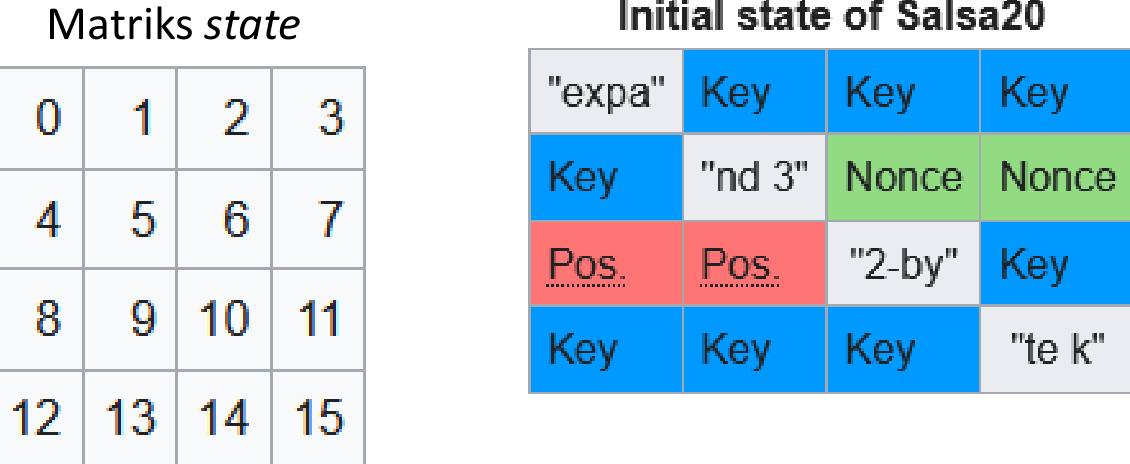
\includegraphics[width=123.69mm,height=127.71mm]{../../images/llm/page_081_img_01.png}%
\end{textblock*}

\end{document}
